
\msection{CROW: Code Randomization of WebAssembly}
\label{section:crow}
\renewcommand{\tool}{CROW\xspace}

%LLVM is a compound of three main components \cite{llvmofficialweb}. 
%First, the frontend (compilers such as clang and rustc) converts the program source code to LLVM intermediate representation (LLVM IR). 
%Second, optimization and transformation processes improve the LLVM IR. 
%Third and final, the backend component is in charge of generating the target Instruction Set.
This section details CROW \cite{CROW}, represented as the red squared tooling in \autoref{fig:approach_landscape}. 
CROW is designed to produce semantically equivalent \wasm variants from the output of an LLVM front-end, utilizing a custom Wasm LLVM backend.

\autoref{diagrams:crow} illustrates CROW's workflow in generating program variants, a process compound of two core stages: \textit{exploration} and \textit{combining}. 
During the \textit{exploration} stage, CROW processes every instruction within each function of the LLVM input, creating a set of functionally equivalent code variants. 
This process ensures a rich pool of options for the subsequent stage.
In the \textit{combining} stage, these alternatives are assembled to form diverse LLVM IR variants, a task achieved through the exhaustive traversal of the power set of all potential combinations of code replacements. 
The final step involves the custom Wasm LLVM backend, which compiles the crafted LLVM IR variants into \wasm binaries. 


%All our implementation choices are based on one premise: \emph{each design decision should increase the number of \wasm\ variants that CROW creates.}
%\subsection*{Overview}

\begin{figure*}[h]
    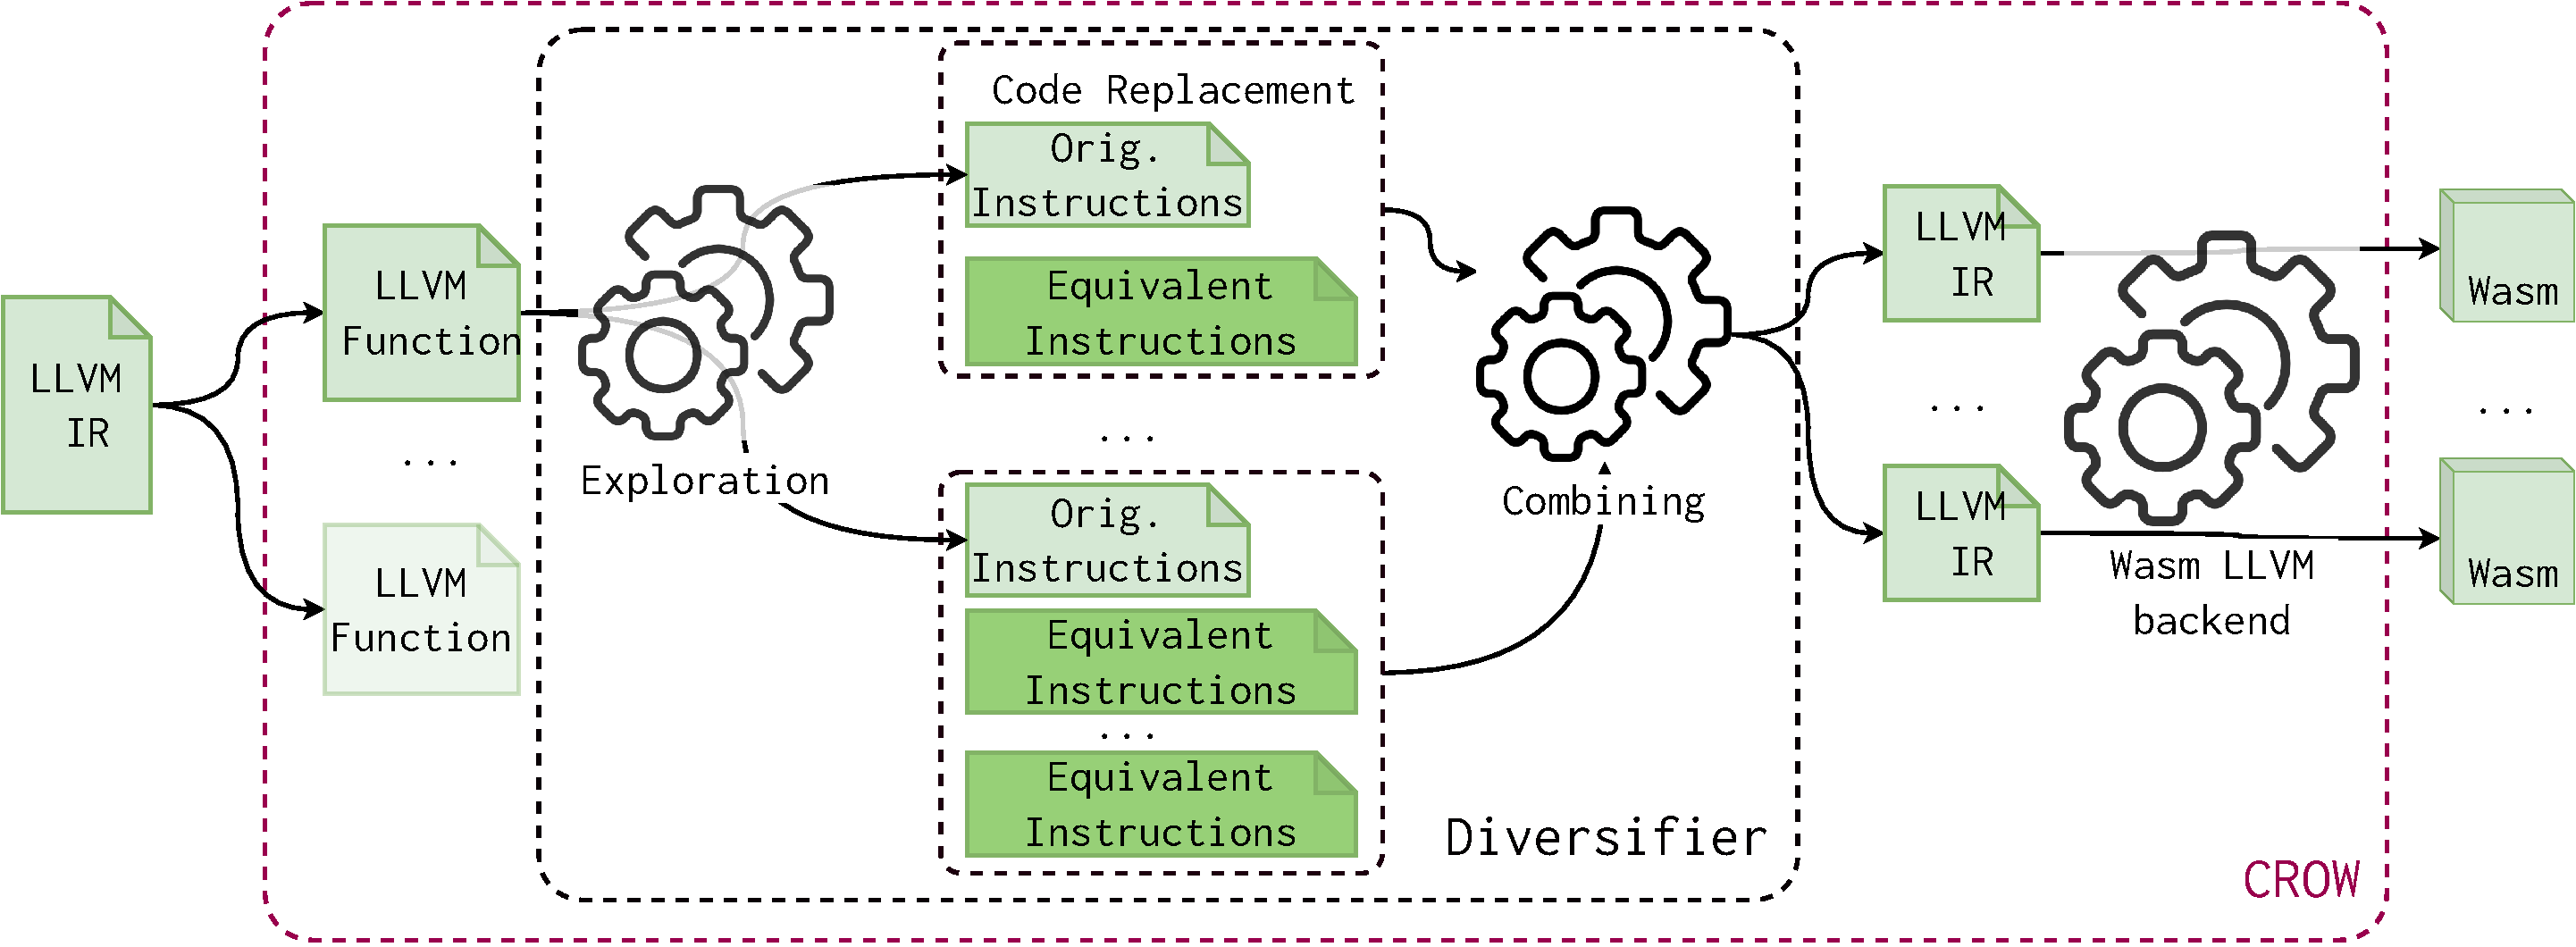
\includegraphics[width=\linewidth]{diagrams/generation/crow.drawio.pdf}
    \caption{CROW components following the diagram in \autoref{fig:approach_landscape}. CROW takes LLVM IR to generate functionally equivalent code replacements. Then, CROW assembles program variants by combining them. Figure taken from \cite{Lic}.}
    \label{diagrams:crow}
\end{figure*}


%CROW operates at the code block level, taking them from the functions defined inside the input LLVM bitcode module. 
%In addition, the retargeted superoptimizer is in charge of finding the potential places in the original code blocks where a replacement can be applied. Finally, we use the enumerative synthesis strategy of the retargeted superoptimizer to generate code replacements.
%The code replacements generated through synthesis are verified, according to \autoref{def:functional-equivalence}, by internally using a theorem prover. 

%\emph{Exploration}
\msubsection{Variants' generation}

The primary component of CROW's exploration process is its code replacements generation strategy. The diversifier implemented in CROW is based on the proposed superdiversifier methodology of Jacob \etal \cite{jacob2008superdiversifier}.
A superoptimizer focuses on \emph{searching} for a new program that is faster or smaller than the original code while preserving its functionality.
The concept of superoptimizing a program dates back to 1987, with the seminal work of Massalin \cite{Massalin1987} which proposes an exhaustive exploration of the solution space. The search space is defined by choosing a subset of the machine's instruction set and generating combinations of optimized programs, sorted by code size in ascending order. If any of these programs is found to perform the same function as the source program, the search halts. On the contrary, a superdiversifier keeps all intermediate search results despite their performance. 


% This paragraph is hard to read
% How Souper works and why we can modify if
% Souper works as follows.
We build CROW upon an already existing superoptimizer for LLVM called Souper \cite{Sasnauskas2017Souper:Superoptimizer}.
Yet, we modify it  to keep all possible solutions in their searching algorithm.
Souper builds a Data Flow Graph for each LLVM integer-returning instruction. 
Then, for each Data Flow Graph, Souper exhaustively builds all possible expressions from a subset of the LLVM IR language.
Each syntactically correct expression in the search space is semantically checked versus the original with a theorem solver. Souper synthesizes the replacements in increasing size. Thus, the first found equivalent transformation is the optimal replacement result of the searching. 
CROW keeps more equivalent replacements during the searching by removing the halting criteria. Instead the original halting conditions, CROW does not halt when it finds the first replacement. CROW continues the search until a timeout is reached or the replacements grow to a size larger that a predefined threshold. 

Notice that the searching space increases exponentially with the size of the LLVM IR language subset. Thus,
we prevent Souper from synthesizing instructions with no correspondence in the \wasm\ backend. This decision reduces the searching space. For example, creating an expression having the  \texttt{freeze} LLVM instructions will increase the searching space for instruction without a Wasm's opcode in the end.
Moreover, we disable the majority of the pruning strategies of Souper for the sake of more program variants.
For example, Souper prevents the generation of the commutative operations during the searching.
On the contrary, CROW still uses such transformation as a strategy to generate program variants. 


The last stage involves the custom Wasm LLVM backend, which is in charge of generating the \wasm programs.
For it, we have the premise of removing all built-in optimizations in the LLVM backend that could reverse Wasm variants.
We disable all optimizations in the \wasm\ backend that could reverse the CROW transformations.

\msubsection{Constant inferring}
\label{CROW:constant_inferring}
CROW, through using Souper adds a new transformation strategy that lead to more \wasm program variants, \emph{constant inferring}.
This means that Souper infers pieces of code as a single constant assignment. 
In particular, Souper focuses on variables that are used to control branches.
% By extending Souper as a superdiversifier, we add this transformation strategy as a new mutation strategy to the ones defined in \autoref{sota:sota}. 
After a \emph{constant inferring}, the generated program is considerably different from the original program, being suitable for diversification.


Let us illustrate the case with an example.
The Babbage problem code in \autoref{babbage} is composed of a loop that stops when it discovers the smaller number that fits with the Babbage condition in Line 4.


{


\begin{minipage}[t]{0.42\linewidth}
        \lstset{
        language=C,
        style=CStyle,
        columns=fullflexible,
        breaklines=true,
        belowcaptionskip=30pt,
        abovecaptionskip=1pt,
        columns=fullflexible,
        breaklines=true, 
        caption={Babbage problem. Taken from \cite{Lic}.},
        frame=b,
        captionpos=b,
        label=babbage,
        postbreak=\mbox{\textcolor{red}{$\hookrightarrow$}\space}
    } 
    \begin{lstlisting}[numbers=left]
    int babbage() {
        int current = 0,
            square;
        while ((square=current*current) % 1000000 != 269696) {
            current++;
        }
        printf ("The number is %d\n", current);
        return 0 ;
    }
    \end{lstlisting}
\end{minipage}
\begin{minipage}[t]{0.48\linewidth}
        \lstset{
        language=C,
        style=CStyle,
        columns=fullflexible,
        breaklines=true,
        belowcaptionskip=3pt,
        abovecaptionskip=1pt,
        columns=fullflexible,
        breaklines=true, 
        frame=b,
        captionpos=b,
        caption={Constant inferring transformation over the original Babbage problem in \autoref{babbage}. Taken from \cite{Lic}.},
        label=inferring,
        postbreak=\mbox{\textcolor{red}{$\hookrightarrow$}\space}
    } 
    \begin{lstlisting}[]
int babbage() {
    @int current = 25264;@
    
    




    printf ("The number is %d\n", current);
    return 0 ;
}
    \end{lstlisting}
\end{minipage}
}
% llvm-opt: rool unroll
In theory, this value can also be inferred by unrolling the loop the correct number of times with the LLVM toolchain.
However, standard LLVM tools cannot unroll the \texttt{\textbf{while}}-loop because the loop count is too large.
% Souper
The original Souper deals with this case, generating the program in \autoref{inferring}. It infers the value of \texttt{current} in Line 2 such that the Babbage condition is reached. Therefore, the condition in the loop will always be false. Then, the loop is dead code and is removed in the final compilation. 
The new program in \autoref{inferring} is remarkably smaller and faster than the original code. Therefore, it offers differences both statically and at runtime\footnote{ Notice that for the sake of illustration, we show both codes in C language, this process inside CROW is performed directly in LLVM IR.}
%  Also, notice that the two programs in the example follow the definition of \emph{functional equivalence} discussed in \autoref{sota:sota}.}


\begin{comment}

\todo{This seems to be out of place :)}
During the implementation of CROW, we have the premise of removing all built-in optimizations in the LLVM backend that could reverse Wasm variants.
Therefore, we modify the \wasm\ backend.
We disable all optimizations in the \wasm\ backend that could reverse the CROW transformations.
\begin{itemize}
    \item Constant folding: this optimization calculates the operation over two (or more) constants in compiling time, and replaces the original expression by its constant result. For example, let us suppose \texttt{$a = 10 + 12$} a subexpression to be compiled, with the original optimization, the \wasm~ backend replaces it by \texttt{$a = 22$}.
    
    \item Expressions normalization: in this case, the comparison operations are normalized to its complementary operation, e.g. \texttt{$a > b$} is always replaced by \texttt{$b <= a$}.
    
    \item Redundant operation removal: expressions such as the multiplication of variables by \texttt{$a = b2^n$} are replaced by shift left operations \texttt{$a = b << n$}.  
\end{itemize}
\end{comment}


\msubsection{Combining replacements}

When we retarget Souper, to create variants, we recombine all code replacements, including those for which a constant inferring was performed.
This allows us to create variants that are also better than the original program in terms of size and performance. Most of the Artificial Software Diversification  works generate variants that are as performant or iller than the original program. By using a superdiversifier, we could be able to generate variants that are better, in terms of performance, than the original program. This will give the option to developers to decide between performance and diversification without sacrificing the former. 

On the other hand, when Souper finds a replacement, it is applied to all equal instructions in the original LLVM binary. In our implementation, we apply the transformations one by one. 
For example, if we find a replacement that is suitable for $N$ difference places in the original program, we generate $N$ different programs by applying the transformation in only one place at a time. Notice that this strategy provides a combinatorial explosion of program variants as soon as the number of replacements increases.



\msubsection{CROW instantiation}
\label{section:crow:example}
%In \autoref{section:crow} we describe the main components and contributions of CROW. In this section we instantiate the workflow presented in \autoref{workflow} from the input of an example C code to the generation of a pool of \wasm\ program variants.

Let us illustrate how CROW works with the example code in \autoref{CExample}. The \texttt{f} function calculates the value of $2 * x + x$ where \texttt{x} is the input for the function.  CROW compiles this source code and generates the intermediate LLVM bitcode in the left most part of \autoref{example:crow:original:llvm}. CROW potentially finds two integer returning instructions to look for variants, as the right-most part of \autoref{example:crow:original:llvm} shows.

% snippet of code showing the detection of code blocks
\begin{minipage}[t]{.9\linewidth}
%\begin{code}
    \lstset{
        language=C,
        basicstyle=\small\ttfamily,captionpos=b,caption={C function that calculates the quantity $2x + x$.},label=CExample, frame=b}
    
    \begin{lstlisting}[style=CStyle]
int f(int x) { 
    return 2 * x + x; 
}    
    \end{lstlisting}
%\end{code}
\end{minipage}

\lstdefinelanguage{LLVM}
    {morekeywords={i32,mul,align,nsw,add,load,store,define,br, ret, shl, ret},
    sensitive=false,
    morecomment=[l]{;},
    morecomment=[s]{;}{;},
    morestring=[b],
}

\lstdefinestyle{nccode}{
    numbers=left,
    tabsize=4,
    showspaces=false,
    breaklines=true, 
    showstringspaces=false,
    moredelim=**[is][{\btHL[fill=black!10]}]{`}{`},
    moredelim=**[is][{\btHL[fill=celadon!40]}]{!}{!}
}
\lstset{
    language=LLVM,
    style=nccode,
    %basicstyle=\small\ttfamily,
    columns=fullflexible,
    breaklines=true
}

\begin{minipage}[t]{0.9\linewidth}
    
    \lstset{numbers=none}
    \noindent\begin{minipage}[t]{.34\linewidth}
    \centering
    \begin{lstlisting}[xleftmargin=1em,escapechar=?]
    define i32 @f(i32) {

      %2 = mul nsw i32 %0,2
      %3 = add nsw i32 %0,%2 

      ret i32 %3
    }
    
    define i32 @main() {
      %1 = tail call i32 @f(i32 10)
      ret i32 %1
    }
    \end{lstlisting}
    \end{minipage}%\hfill%
    \begin{minipage}[t]{.32\linewidth}
        \begin{lstlisting}[xleftmargin=1em,escapechar=?]
?Replacement candidates for code\_1?

`%2 = mul nsw i32 %0,2`

!%2 = add nsw i32 %0,%0!

!%2 = shl nsw i32 %0, 1:i32!
    \end{lstlisting}
    \end{minipage}%\hfill%
    \begin{minipage}[t]{.32\linewidth}
        \lstdefinestyle{nccode}{
        tabsize=4, 
        showspaces=false,
        breaklines=true, 
        showstringspaces=false,
        moredelim=**[is][{\btHL[fill=black!10]}]{`}{`},
        moredelim=**[is][{\btHL[fill=celadon!40]}]{!}{!}
        }
        \lstset{
            language=LLVM,
            style=nccode,
            columns=fullflexible,
            breaklines=true,
            belowcaptionskip=1pt,
            abovecaptionskip=1pt,
        } 
        \begin{lstlisting}[name={B},escapechar=?]
?Replacement candidates for code\_2?

`%3 = add nsw i32 %0,%2`

!%3 = mul nsw %0, 3:i32!
        \end{lstlisting}
    \end{minipage}
    \centering
    \hrule
    \vspace{2mm}
    \captionof{lstlisting}{LLVM's intermediate representation program, its extracted instructions and replacement candidates. Gray highlighted lines represent original code, green for code replacements. }\label{example:crow:original:llvm}
\end{minipage}

\begin{minipage}[t]{.9\linewidth}
    \lstset{numbers=none}
    \noindent\begin{minipage}[t]{.5\linewidth}
    \begin{lstlisting}[xleftmargin=1em,escapechar=?]
`%2 = mul nsw i32 %0,2`
`%3 = add nsw i32 %0,%2`

!%2 = add nsw i32 %0,%0!
`%3 = add nsw i32 %0,%2`

!%2 = shl nsw i32 %0, 1:i32!
`%3 = add nsw i32 %0,%2`

    \end{lstlisting}
    \end{minipage}%\hfill%
    \begin{minipage}[t]{.5\linewidth}
        \lstdefinestyle{nccode}{
        tabsize=4, 
        showspaces=false,
        breaklines=true, 
        showstringspaces=false,
        moredelim=**[is][{\btHL[fill=black!10]}]{`}{`},
        moredelim=**[is][{\btHL[fill=celadon!40]}]{!}{!},
        moredelim=**[is][{\btHL[fill=weborange!40]}]{'}{'}
        }
        \lstset{
            language=LLVM,
            style=nccode,
            columns=fullflexible,
            breaklines=true,
            belowcaptionskip=1pt,
            abovecaptionskip=1pt,
        } 
        \begin{lstlisting}[xleftmargin=1em,escapechar=?]
'%2 = mul nsw i32 %0,2'
!%3 = mul nsw %0, 3:i32!

'%2 = add nsw i32 %0,%0'
!%3 = mul nsw %0, 3:i32!

'%2 = shl nsw i32 %0, 1:i32'
!%3 = mul nsw %0, 3:i32!

    \end{lstlisting}
    \end{minipage}
    \centering
    \hrule
    \vspace{2mm}
    \captionof{lstlisting}{Candidate code replacements combination. Orange highlighted code illustrate replacement candidate overlapping.}\label{example:crow:original:combination}
\end{minipage}


    

CROW, detects \texttt{code\_1} and \texttt{code\_2} as the enclosing boxes in the left most part of \autoref{example:crow:original:llvm} shows. CROW synthesizes $2 + 1$ candidate code replacements for each code respectively as the green highlighted lines show in the right most parts of \autoref{example:crow:original:llvm}.
The baseline strategy of CROW is to generate variants out of all possible combinations of the candidate code replacements, \ie uses the power set of all candidate code replacements.

In the example, the power set is the cartesian product of the found candidate code replacements for each code block, including the original ones, as \autoref{example:crow:original:combination} shows. The power set size results in $6$ potential function variants. Yet, the generation stage would eventually generate $4$ variants from the original program. CROW generated 4 statically different Wasm  files, as \autoref{example:crow:variants:wasm} illustrates. This gap between the potential and the actual number of variants is a consequence of the redundancy among the bitcode variants when composed into one. In other words, if the replaced code removes other code blocks, all possible combinations having it will be in the end the same program. In the example case, replacing \texttt{code\_2} by \texttt{mul nsw \%0, 3}, turns \texttt{code\_1} into dead code, thus, later replacements generate the same program variants. The rightmost part of \autoref{example:crow:original:combination} illustrates how for three different combinations, CROW produces the same variant. We call this phenomenon a \emph{code replacement overlapping}.

\lstdefinestyle{nccode}{
        numbers=none,
        firstnumber=2,
        stepnumber=1,
        numbersep=10pt,
        tabsize=4, 
        showspaces=false,
        breaklines=true, 
        showstringspaces=false,
    moredelim=**[is][\btHL]{`}{`},
    moredelim=**[is][{\btHL[fill=black!10]}]{`}{`},
    moredelim=**[is][{\btHL[fill=celadon!40]}]{!}{!}
}

\lstset{
    language=WAT,
    style=nccode,
    basicstyle=\footnotesize\ttfamily,
    columns=fullflexible,
    breaklines=true
}


\begin{minipage}[t]{0.9\linewidth}
    \lstset{numbers=none}
    \noindent\begin{minipage}[t]{.45\linewidth}
    \begin{lstlisting}[xleftmargin=1em,escapechar=?]
func $f (param i32) (result i32)
   local.get 0
    `i32.const 2`
    `i32.mul`
    `local.get 0`
    `i32.add`

        \end{lstlisting}
\begin{lstlisting}[xleftmargin=1em,escapechar=?]
func $f (param i32) (result i32)
    local.get 0
    !local.get 0!
    !i32.add!
    `local.get 0`
    `i32.add`

                \end{lstlisting}
    \end{minipage}\hfill
    \noindent\begin{minipage}[t]{.45\linewidth}
\begin{lstlisting}[xleftmargin=1em,escapechar=?]
func $f (param i32) (result i32)
    local.get 0
    !i32.const 1!
    !i32.shl!
    `local.get 0`
    `i32.add`

    \end{lstlisting}
\begin{lstlisting}[xleftmargin=1em,escapechar=?]
func $f (param i32) (result i32)
    local.get 0
    !i32.const 3!
    !i32.mul!

        \end{lstlisting}
    \end{minipage}

    \centering
    \hrule
    \vspace{2mm}
    \captionof{lstlisting}{Wasm  program variants generated from program \autoref{CExample}.}\label{example:crow:variants:wasm}
\end{minipage}




One might think that a reasonable heuristic could be implemented to avoid such overlapping cases. Instead, we have found it easier and faster to generate the variants with the combination of the replacement and check their uniqueness after the program variant is compiled. This prevents us from having an expensive checking for overlapping inside the CROW code. Still, this phenomenon calls for later optimizations in future works.



\begin{tcolorbox}[title=Contribution paper and artifact,boxrule=1pt,arc=.2em,boxsep=1.0mm]
   CROW fully presented in Cabrera-Arteaga \etal "CROW: Code Randomization of WebAssembly"
    \emph{Network and Distributed System Security Symposium, MADWeb}
    \url{https://doi.org/10.14722/madweb.2021.23004}.
    \\\\
    CROW source code is available at \url{https://github.com/ASSERT-KTH/slumps}

\end{tcolorbox}

